%every chapter wil be split into a new document. For the sake of the structure, this one_doc strategy is held up
\chapter{Application Area and Goals}
\label{cha:area_goals}
\textcolor{red}{\textit{Do we write a Management summary?}}\\
This paper represents a documentation for the data mining project "Mining the Success for Movies". Information in this paper refers to the (sample) dataset and python scripts handed in for a classification problem. The structure of this paper is as follows: Chapter \ref{cha:area_goals} provides an overview of the problem the project is based on. Goals of the project and the theoretical framework will be discussed as well. Chapter \ref{cha:data_selection} deals with the structure and size of the data. Here, a closer look will be taken at the dataset at hand. Questions that had to be answered were for example which information were provided in the original dataset or which problems were identified concerning for instance outliers or missing values. Chapter \ref{cha:preprocessing_transformation} explains which preprocessing steps had to be taken in order to cleanse the dataset and to prepare it for the data mining step. Chapter \ref{cha:data_mining} describes which data mining techniques regarding algorithms and parameters were used to learn an expedient model in respect of the goals set in Chapter \ref{cha:area_goals}. Chapter \ref{cha:interpretation_evaluation} closes this paper by describing which insights could be won for the problem at hand. Here, a critical reflection is delineated how the model could be improved further in order to provide even more precise results.

\section{Problem Statement}
Already well before new movies are being produced, every stakeholder certainly is interested in the monetary success of the given movie. In order to predict the success costly methods are being applied, such as market investigations. \textcolor{red}{\textit{Do we need a source? koennte noch ausgefuehrt werden.}}

The benefit Data Mining brings to the analysis of large datasets, can also be transferred onto the stated problem of predicting a movie's success. Based on given data of already released movies, a model is being learned which shall be applied on upcoming or planned movies. In order to learn and apply the model various pieces of information are taken into account. Just a few are budget, revenues, runtime, genre and information on the release. Information on the dataset and on all preprocessing methods which were applied will be provided in chapter \ref{cha:data_selection}.

\section{Goals}
The goal of this project is to learn a model which will predict how successful a not yet released movie will be. This is done by using common data mining techniques in Python. As a main objective the question \textit{"Based on revenue, will the movie be popular or will it be a flop?"} shall be answered for all possible combinations of information on a new movie as precisely as possible.
In order to be as precisely as possible, not only different algorithms are being tested, but also parameter tuning is being applied with different performance measures \footnote{Further information on applied techniques and evaluation methods is provided in chapter \ref{cha:data_mining}}.


\begin{itemize}
	\item Problem Statement and idea behind the project
	\item General introduction similar to Project outline
\end{itemize}

\section{Theoretical framework}
\begin{itemize}
	\item keep it small
	\item roughly 1 Page
\end{itemize}
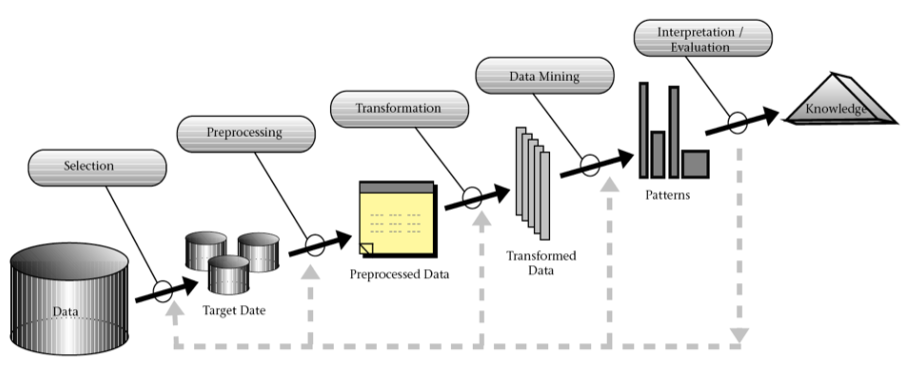
\includegraphics[width=\textwidth]{images/DM_Process.png}








